\documentclass[conference]{IEEEtran}
\IEEEoverridecommandlockouts
% The preceding line is only needed to identify funding in the first footnote. If that is unneeded, please comment it out.
\usepackage{amsmath,amsthm,amssymb} %modos matemáticos y  simbolos
\usepackage{latexsym,amsfonts} %simbolos matematicos
\usepackage{cancel} %hacer la linea que cancela las ecuaciones
\usepackage[spanish, es-noshorthands]{babel} %comandos en español y cambia el cuadro por la tabla
\decimalpoint %cambia las comas por puntos decimal
\usepackage[utf8]{inputenc} %caracteristicas del español
\usepackage{physics} %Simbolos fisicos
\usepackage{array} %mejores formatos de tabla
\parindent =0cm %sangria 
\usepackage{algorithmic}
\usepackage{graphicx}
\usepackage{textcomp}
\usepackage{xcolor}
\usepackage{mathtools} 
\usepackage[framemethod=TikZ]{mdframed}%Entornos talegas
\usepackage[colorlinks = true,
			linkcolor = blue,
			citecolor = black,
			urlcolor = blue]{hyperref}%formato de los links y URL's
\usepackage{multicol} %varias columnas
\usepackage{enumerate} %enumeraciones
\usepackage{pgf,tikz,pgfplots} %documentos en formato tikz
\usepackage{mathrsfs} %letras chingonas (transformada de laplace)
\usepackage{subfigure} %varias figuras seguidas
\usepackage{tabulary}
\usepackage{multirow} %ocupar varias filas en una tabla
\usepackage{fancybox} %recuadros talegas
\usepackage{float} %ubicar graficas
\usepackage{color}
\usepackage{comment}
\usepackage{stackrel}
\usepackage{calligra}
\usepackage{lipsum}
\usepackage{cite}
\pgfplotsset{compat=1.16} 

\newcommand{\R}{\mathbb{R}}
\newcommand{\Z}{\mathbb{Z}}
%%%%%%%%%%%%%%%%%%%%%%%%%%%%%%%%%%%%%%%%%%%%%%%%%%%%%%
\def\BibTeX{{\rm B\kern-.05em{\sc i\kern-.025em b}\kern-.08em
    T\kern-.1667em\lower.7ex\hbox{E}\kern-.125emX}}
\begin{document}

\title{Eficiencia de un Detector Geiger-Müller \\
{\footnotesize \scshape{Proyecto Final}}
}

\author{\IEEEauthorblockN{1\textsuperscript{st} Diego Sarceño Ramírez}
\IEEEauthorblockA{\textit{201900109} 
}
%\and
%\IEEEauthorblockN{2\textsuperscript{nd} Andrés Pérez}
%\IEEEauthorblockA{\textit{201704199}
%}
%\and
%\IEEEauthorblockN{3\textsuperscript{rd} Diego Sarceño Ramírez}
%\IEEEauthorblockA{\textit{201900109} \\
%}
}



\maketitle

\begin{abstract}
	En este artículo se presenta una simulación realizada en GEANT4 de un detector Geiger-Müller, con el fin de medir la eficiencia en energía, geométrica y total del mismo. Para ello se realizó el sistema de cilindros del detector con cloro molecular. Los resultados de esta simulación no fueron los esperados por desperfectos en el programa, en concreto, con los detectores.
\end{abstract}

\begin{IEEEkeywords}
	Detector Geiger-Müller, contador Geiger, radiaciones ionizantes, radiactividad.
\end{IEEEkeywords}

%\section{Objetivos}
%
%\subsection{General}
%    \begin{enumerate}[1.]
%        \item Realizar un circuito sumador/restador de 3 bits de entrada con una salida de resultado en un display de 7 segmentos en formato base 10.
%    \end{enumerate}
%\subsection{Específicos}
%    \begin{enumerate}
%        \item Diseñar múltiples circuitos combinacionales para obtener un resultado único en conjunto.
%        \item Implementar un circuito de lógica combinacional capaz de realizar operaciones aritméticas simples utilizando únicamente compuertas lógicas.
%        \item Optimizar el uso de compuertas mediante técnicas distintas al uso de Mapas de Karnaugh.
%        \item Contrastar los diseños teóricos con los resultados experimentales de los circuitos implementados físicamente.
%    \end{enumerate}
%\section{Introducción}
    
\section{Marco Teórico}


Un detector Geiger-Müller es un dispositivo utilizado para detectar y medir la radiación ionizante, como los rayos gamma y los rayos $X$, así como partículas alfa y beta. Recibe su nombre de los físicos alemanes Hans Geiger y Walther Müller, quienes desarrollaron este tipo de detector en la década de 1920.

El funcionamiento básico de un detector Geiger-Müller se basa en el principio de ionización secundaria. Consiste en un tubo lleno de un gas a baja presión, generalmente argón o helio, y contiene un electrodo central metálico cargado positivamente y un cilindro externo cargado negativamente. Cuando una partícula o un fotón ionizante atraviesa el tubo, provoca la ionización de los átomos del gas. La ionización produce electrones libres y iones positivos.

El detector Geiger-Müller cuenta con un circuito de detección e incluye un contador para contar y mostrar el número de partículas o fotones detectados por unidad de tiempo. Es importante tener en cuenta que los detectores Geiger-Müller son sensibles a la radiación ionizante, pero no proporcionan información detallada sobre la energía o el tipo de partícula. Por lo tanto, se utilizan principalmente para detectar la presencia de radiación y obtener una medida aproximada de su nivel.

Los detectores Geiger-Müller se utilizan ampliamente en aplicaciones donde se necesita una detección rápida y sencilla de la radiación, como en la monitorización de la radiación en entornos nucleares, la detección de fugas radiactivas, la radiografía industrial y la investigación científica.



%\section{Diseño Experimental}



\section{Montaje Experimental}
%    \subsection{Materiales a Utilizar}
%        \begin{itemize}
%    	\item 
%    \end{itemize}
%
%    \subsection{Procedimientos}
%        \begin{enumerate}
%            \item 
%        \end{enumerate}
\subsection{Diseño de Simulación}
Esta simulación consiste en una fuente cilíndrica delgada que será colocada de forma coaxial a un detector también de geometría cilíndrica (ver figura \ref{detector}). Todos os elementos de la simulación estarán dentro de un entorno de aire. La fuente no se considerará de un material específico, mas bien, será una región desde la cual se emiten los rayos gamma. El detector simulará las condiciones de un Geiger-Müller de geometría cilíndrica, consistiendo en un envoltorio cilíndrico de acero inoxidable con una ventana del mismo material en uno de sus extremos. El gas de relleno de la cavidad interna del detector será cloro molecular, que es un halógeno. La fuente será colocada a $5cm$ del extremo del detector donde se encuentra la ventana (ver medidas en figura \ref{lateral}).
        
\begin{figure}[H]
	\centering
	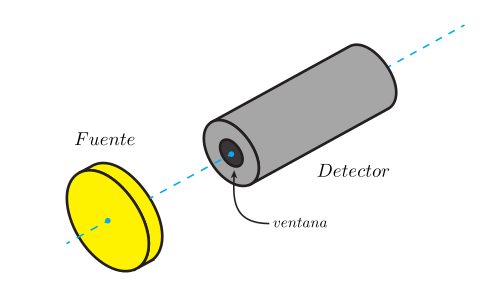
\includegraphics[scale=0.4]{./Imagenes/detector.png}
	\caption{Esquema del montaje.}
	\label{detector}
\end{figure}


\begin{figure}[H]
	\centering
	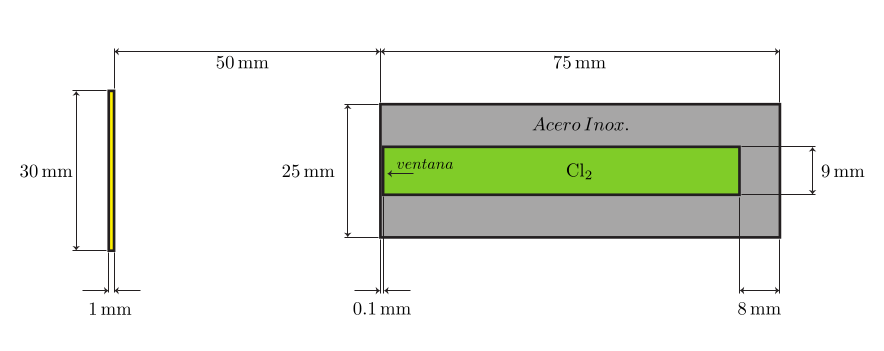
\includegraphics[scale=0.25]{./Imagenes/lateral.png}
	\caption{Vista lateral.}
	\label{lateral}
\end{figure}
        

\subsection{Datos a Medir}
Se considerará que un rayo gamma es detectado, si este produce un electrón por medio de alguna interacción con el gas de cloro.

\subsubsection{Eficiencia en Energía}
Sea $n_\gamma (E)$ el número de rayos detectados y $N_\gamma (E)$ el número de rayos emitidos por la fuente para una energía $E$ en el rango $100keV \leq E \leq 1500 keV$. Con esto, la eficiencia en energía se define como:
\begin{equation}
	\epsilon (E) = \frac{n_\gamma (E)}{N_\gamma (E)}. \label{energia}
\end{equation}

\subsubsection{Eficiencia en Geometría}
Ahora, sea $n_\gamma$ el número de rayos que alcanzan el volumen de detección (no interesa si producen interacción) y $N_\gamma$ el número de rayos gamma emitidos por la fuente en todas las direcciónes posibles. Esta eficiencia está definida como:
\begin{equation}
	\epsilon _g = \frac{n_\gamma}{N_\gamma}. \label{geometrica}
\end{equation}

\subsubsection{Eficiencia Total}        
Esta eficiencia depende tanto del montaje como de la geometría del mismo.
\begin{equation}
	\epsilon _T (E) = \epsilon (E) \epsilon _g.	\label{total}
\end{equation}
        
        
        
\section{Resultados}

\begin{figure}[H]
	\centering
	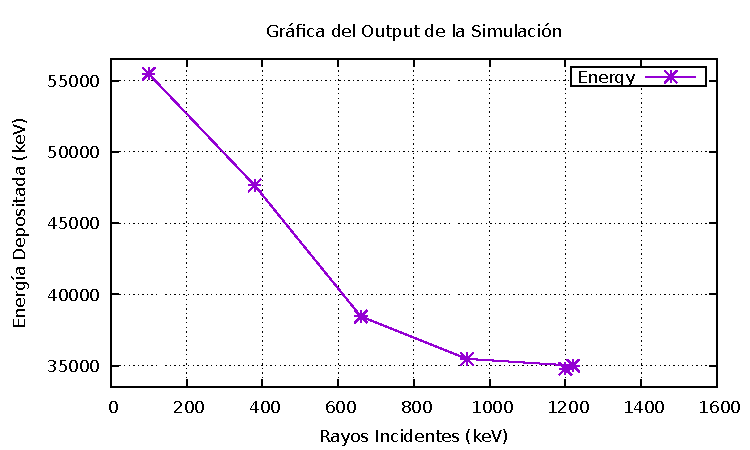
\includegraphics[scale=0.65]{./Codigos/Ajuste.pdf}
	\caption{Gráfica de "Energy deposited per run, in scoring volume" contra la energía del conjunto de rayos gamma.}
	\label{ajuste}
\end{figure}
    
    
\section{Discusión de Resultados}
\begin{enumerate}
    \item Se tomó el \textit{ejemplo 2} dado en clase y se modificó para poder utilizarlo en este sistema en partícular, se modificó el archivo \textit{LA02DetectorConstruction.cc} para hacer el experimento. Esto devuelve resultados inesperados y, practicamente, inaceptables respecto a lo que se esperaba.
    \item Los resultados mostrados son la energía depostiada por cada "run" en el volumen de "hit". Estos resultados se muestran en la gráfica \ref{ajuste} esto se hizo para intentar encontrar una relación entre los resultados obtenidos y la eficiencia en energía \eqref{energia} por medio de la forma de la gráfica.
    \item Estos resultados inconclusos pueden deberse a un malfuncionamiento en el codigo de los detectores, error que no se pudo corregir. O a un "bug" en GEANT4 con esta simulación, dado que es un programa que continuamente da problemas en varios sistemas operativos y/o ordenadores.
\end{enumerate}



\section{Conclusiones}
\begin{enumerate}
    \item Dada la discusión de los resultados y los resultados mostrados, es claro que no se encontró lo esperado. Con esto, podemos concluir que el detector no estaba bien programado y no se detectaban interacciones individuales, sino un resultado colectivo en términos de la energía. Al tener una gráfica descendiente, se podría pensar que la eficiencia también disminuye puesto que se detecta menos energía.
\end{enumerate}






\section{Recomendaciones}
\begin{itemize}
	\item Se recomienda revisar exaustivamente el código de los detectores, ya que con esto se arreglan todos los datos a los esperados para poder utilizar las definiciones de las respectivas eficiencias.
\end{itemize}


\section{Anexos}
\textit{Screenshot} de la simulación realizada.
\begin{figure}[H]
	\centering
	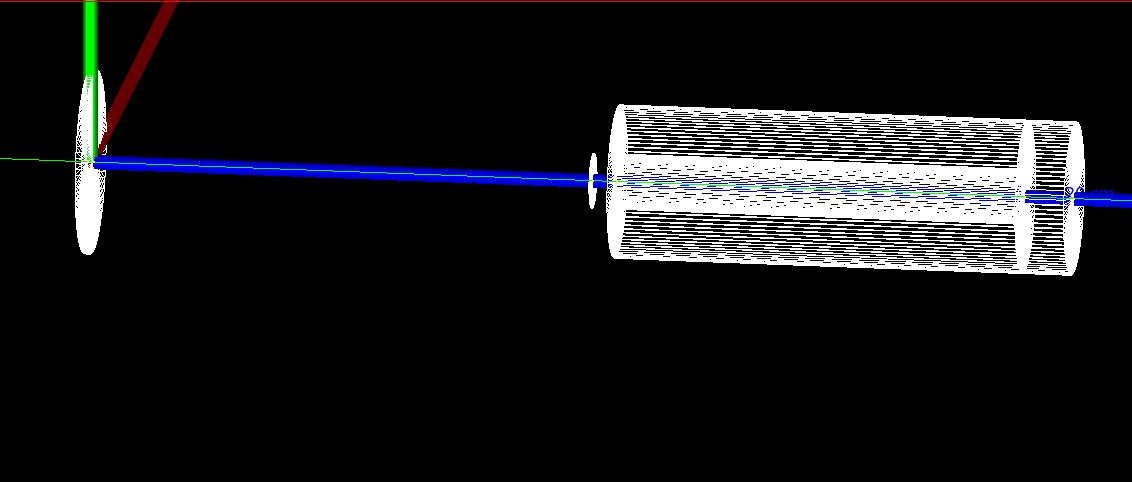
\includegraphics[scale=0.2]{./Imagenes/fig.jpeg}
	\caption{Imagen de la fuente cilíndrica y el detector.}
\end{figure}
        
        
        
\begin{thebibliography}{00}
\bibitem{b1} Lamarsh, J. R., \& Baratta, A. J. (2001). \textit{Introduction to nuclear engineering} (Vol. 3). Upper Saddle River, NJ: Prentice hall.
\bibitem{b2} Lilley, J. (2013). \textit{Nuclear physics: principles and applications.} John Wiley \& Sons.
\end{thebibliography}
\end{document}


